%!TEX root = ../template.tex
%%%%%%%%%%%%%%%%%%%%%%%%%%%%%%%%%%%%%%%%%%%%%%%%%%%%%%%%%%%%%%%%%%%%
%% chapter3.tex
%% NOVA thesis document file
%%
%% Chapter with a short latex tutorial and examples
%%%%%%%%%%%%%%%%%%%%%%%%%%%%%%%%%%%%%%%%%%%%%%%%%%%%%%%%%%%%%%%%%%%%

\typeout{NT FILE chapter3.tex}%

\makeatletter
\newcommand{\ntifpkgloaded}{%
  \@ifpackageloaded%
}
\makeatother


\chapter{System Model \& Software Architecture}\label{cha:system_model}

This chapter provides an in-depth exploration of the system model and software architecture of TTT.\@ We begin by introducing the system's overarching objectives and foundational principles. Next, we define the design goals that guided its development, followed by a detailed exposition of the system model and software architecture. Subsequently, we present the threat model, analyzing the potential threats and adversaries accounted for in TTT's design. Finally, we conclude with a comprehensive summary that synthesizes the key insights discussed throughout the chapter.

\section{TTT Proposal}\label{sec:system_propostal}

As shown previously in \autoref{sec:motivation}, Tor is a widely used anonymity network that provides users privacy and anonymity while browsing the internet. However, advances in machine learning and data analysis have made it possible to de-anonymize Tor users by analyzing their traffic patterns, therefore compromising the privacy and anonymity that Tor aims to provide [REFS AQUI]. 

This can be achieved through some traffic analysis attacks, such as fingerprinting and traffic correlation. As discussed in \autoref{sec:problem}, these traffic analysis attacks represent a significant threat to Tor users' privacy and anonymity, as sophisticated adversaries can use machine learning and artificial intelligence techniques to analyze monitored traffic patterns and de-anonymize users and their browsing activities.

This way, we propose TTT, an extension of Tor source code that includes a differential private scheduler to protect the users' data and prevent de-anonymization attacks. By incorporating Differential Privacy into the Tor network, we have increased the resistance against fingerprinting and correlation attacks. In addition, TTT also introduces a new differential private `Packet Padding Cells' generation mechanisms, which allows hosts to generate additional traffic that can be used to obfuscate the traffic patterns and make it more difficult for adversaries to analyze the traffic.

The main goal is to reinforce Tor's resistance against traffic analysis attacks, specially fingerprinting and correlation, therefore fortifying users' privacy and anonymity, and ensuring that the solution maintains reasonable performance and usability. To achieve this goal, we designed TTT with the following design goals in mind:
\paragraph{Privacy and Anonymity:} The solution must reinforce Tor's resistance against traffic analysis attacks, specifically fingerprinting and correlation attacks. 
\paragraph{Formally Proven:} The solution must be formally proven to provide a certain level of privacy, by using Differential Privacy. This way, we add a new and important layer of security and trust to the Tor network and users.
\paragraph{Tor's Extension:} The solution must be an extension of the Tor project, respecting Tor's design principles and rules. As a very popular open source project, Tor has a large community of users and developers, and it is important to ensure that the solution can be easily integrated into the existing Tor source code. The project contains a set of principles and rules that we must respect.
\paragraph{Compactibility:} The solution must be easily integrated into the existing Tor network, allowing users and hosts to configure the trade-offs between privacy and performance. The Tor network is composed of several voluntary relays, where hosts decide how to configure. Therefore, we must ensure that the solution can be easily integrated into the existing Tor network and compactible with relays that may be unaware of our solution.
\paragraph{Unobservability:} The solution must enhance Tor's resistance against traffic analysis attacks, specifically fingerprinting and correlation attacks, in comparison to the existing Tor network. 
\paragraph{Configurability:} As an extension of the Tor project, the solution must use the existing Tor configuration files and allow users and hosts to configure the trade-offs between privacy and performance. This way, users can choose the level of privacy they want to achieve.
\paragraph{Performance:} We consider that performance is a key aspect of the solution. However, the solution does not aim to improve the performance of the Tor network, but rather to ensure that the solution does not significantly impact the performance of the Tor network. 

\section{System Model}\label{sec:system_model}

As stated previously, the solution is an extension of the Tor project, so the system model is also similar to the Tor system model. The system model is composed by several voluntary relays, which compose the network and are responsible for forwarding the traffic. Clients connect to the network through an entry relay and the traffic is forwarded through a series of relays. The relays are responsible for forwarding the traffic and the scheduler executes the differential private mechanisms to inject jitter or shaft traffic into the network, between relays. 

\begin{figure}[!h]
  \centering
  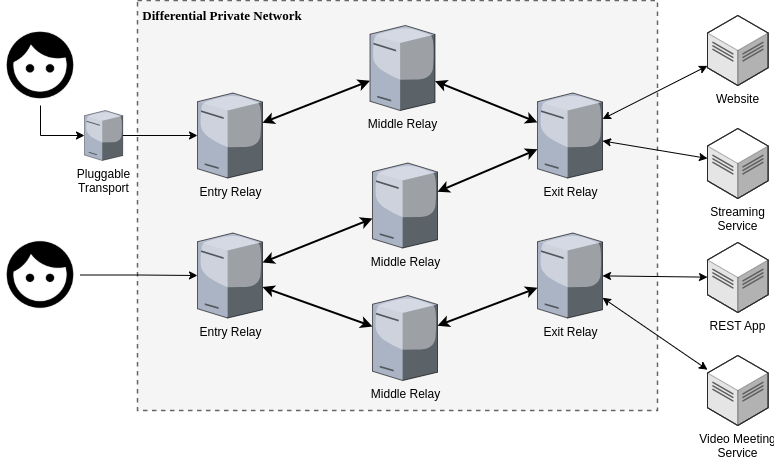
\includegraphics[width=\textwidth]{Chapters/Figures/System_Model_Geral.png}
  \caption{Differential Private Network System Model}\label{fig:system_model}
\end{figure}

\section{Threat Model}\label{sec:threat_model}

TTT is designed to strengthen the Tor network's privacy protections and bolster its defenses against traffic analysis attacks, with a particular focus on fingerprinting and correlation threats. Our threat model assumes State-Level Adversaries are capable of observing Tor users' traffic patterns with the aim of de-anonymization, as illustrated in \autoref{fig:thread_model}. As discussed earlier in \autoref{sec:problem}, we identify traffic analysis as the principal threat to Tor — the very challenge that TTT seeks to address — with fingerprinting and traffic correlation attacks representing the primary vectors.

In shaping our threat model, we closely follow the foundational Tor threat model outlined by~\cite{dingledine2004tor}. Accordingly, we consider adversaries who can monitor portions of network traffic, manipulate data flows, operate their own onion routers, and compromise a fraction of existing routers. The adversary's ultimate objective is the de-anonymization of users and the exposure of their browsing activities.

Moreover, we acknowledge that State-Level Adversaries may collaborate, exchanging information across different segments of the network. Such cooperation enables them to piece together a broader view of the network's traffic, amplifying their capabilities from a single Autonomous System (AS). Nevertheless, our model does not account for the presence of a global adversary capable of observing the entire network.

Building on the original assumptions put forth by~\citeauthor{dingledine2004tor}~\cite{dingledine2004tor}, we consider both passive and active adversaries. A passive adversary merely observes traffic patterns, applying machine learning and data analysis techniques to infer user identities and behaviors. Conversely, an active adversary compromises onion routers to inject traffic into the network — not merely to observe, but to facilitate more sophisticated traffic analysis attacks. Traffic injection, in this context, becomes a strategic tool for the adversary to train machine learning models capable of uncovering users' identities and tracking their navigation through the Tor network.


\begin{figure}
  \centering
  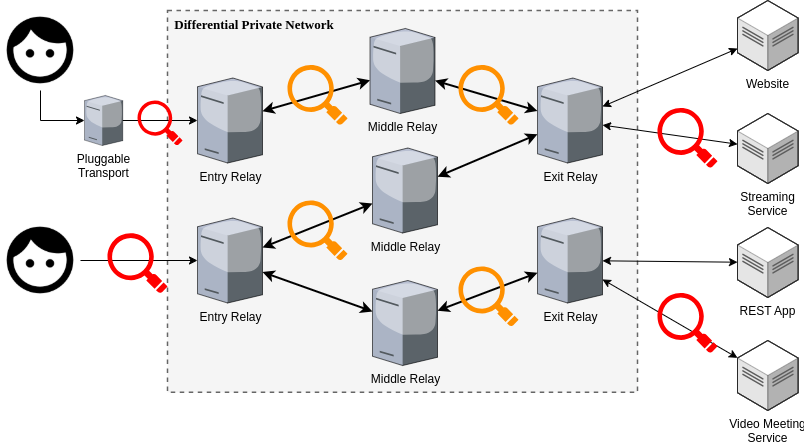
\includegraphics[width=\textwidth]{Chapters/Figures/Threat_Model.png}
  \caption{Threat Model over System Model}\label{fig:thread_model}
\end{figure}

\section{Software Architecture}\label{sec:software_architecture}

\subsection{Tor Kist based Architecture}\label{sec:tor_kist_architecture}

\subsection{TTT Architecture}\label{sec:ttt_architecture}

\section{Parameterization}\label{sec:parameterization}

\subsection{Used Techniques}\label{sec:used_techniques}

\subsection{Jitter Parameterization}\label{sec:jitter_parameterization}

\subsection{Packet Padding Cells Parameterization}\label{sec:packet_padding_parameterization}

\section{Jitter Development Strategy}\label{sec:jitter_development_strategy}

\section{Packet Padding Cells Development Strategy}\label{sec:packet_padding_cells_development_strategy}

\section{Discussion}\label{sec:architeture_discussion}